\documentclass[letterpaper,11pt]{article}
\usepackage{graphicx}
\usepackage{listings}
\usepackage[super]{nth}
\usepackage[hyphens]{url}
\usepackage{hyperref}
\usepackage{amsmath}
\usepackage[makeroom]{cancel}
\usepackage[table]{xcolor}
\usepackage{comment}
\usepackage[space]{grffile}
\usepackage{csvsimple}
\usepackage{longtable}
\usepackage{adjustbox}


\newcommand*{\srcPath}{../src}%

\lstset{
	basicstyle=\footnotesize,
	breaklines=true,
}

\begin{document}

\begin{titlepage}

\begin{center}

\Huge{Assignment 2}

\Large{CS 734:  Introduction to Information Retrieval}

\Large{Fall 2017}

\Large{Grant Atkins}

\Large Finished on \today

\end{center}

\end{titlepage}

\newpage


% =================================
% First question
% =================================
\section*{1}

\subsection*{Question}

\begin{verbatim}
4.1. Plot rank-frequency curves (using a log-log graph) for 
words and bigrams in the Wikipedia collection available through 
the book website (http://www.searchengines-book.com). Plot a 
curve for the combination of the two. What are the best 
values for the parameter c for each curve?
\end{verbatim}

\subsection*{Answer}

For this question I wrote two files of code, \textbf{rankFreq.py} and \textbf{rankFreq.R} in with the ``small'' wiki dataset provided from the textbooks website . 
The first python file iterates through all of the wiki html files, tokenizes them, finds token frequency, and then writes them to a CSV in descending frequency order.
To retrieve the text from each of the html files I used Beautifulsoup. 
It should be noted when retrieving each token from the html files I did not take into account uppercase or lowercase as same terms, I treated them as different and more than probably affected the outcome of this answer.
After the code tokenizing the terms it created a list of unigrams and bigrams for all the terms keeping them in separate lists to count frequencies.
I used the NLTK python library to make bigram pairs.
The code for this is shown below in Listing \ref{lst:q1py}.
The top 10, ranked by token frequency, results are shown below in Figures \ref{fig:q1uni} and \ref{fig:q1bi}.
The full CSV files can be found in my Github repository \cite{github}.
Without removing stop words its apparent that words like ``the'' and ``of'' would some of the top unigram and bigram pairs.

 \lstinputlisting[frame=single,caption={Python script to tokenize and find frequencies and calculate C parameters},label=lst:q1py,captionpos=b,numbers=left,showspaces=false,showstringspaces=false,basicstyle=\footnotesize]{\srcPath/rankFreq.py}
 
 To create the graphs I used R's ggplot2 library. 
 The code to create these graphs is shown in Listing \ref{lst:q1R}.
 The figures created from the afore mentioned code are shown in Figure \ref{fig:q1p1}, \ref{fig:q1p2}, and \ref{fig:q1p3}.
For unigrams the best \textit{C} parameter was 0.14, while for bigrams it was 0.1.
 
  \lstinputlisting[frame=single,caption={Python script to tokenize and find frequencies and calculate C parameters},label=lst:q1R,captionpos=b,numbers=left,showspaces=false,showstringspaces=false,basicstyle=\footnotesize]{\srcPath/rankFreq.R}

  \begin{figure}[h]
  \centering
  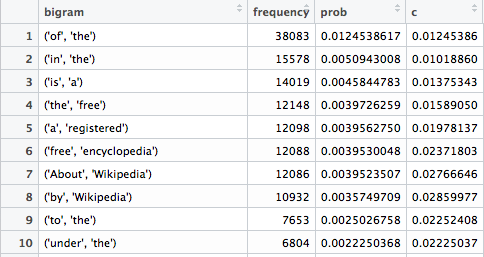
\includegraphics[scale=0.6]{unigram_10.png}
  \caption{Top 10 unigrams found}
  \label{fig:q1uni}
  \end{figure}

  \begin{figure}[h]
  \centering
  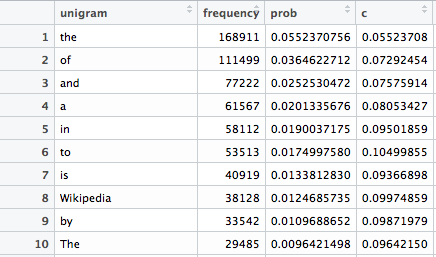
\includegraphics[scale=0.6]{bigram_10.png}
  \caption{Top 10 bigrams found}
  \label{fig:q1bi}
  \end{figure}
  
   \begin{figure}[h]
  \centering
  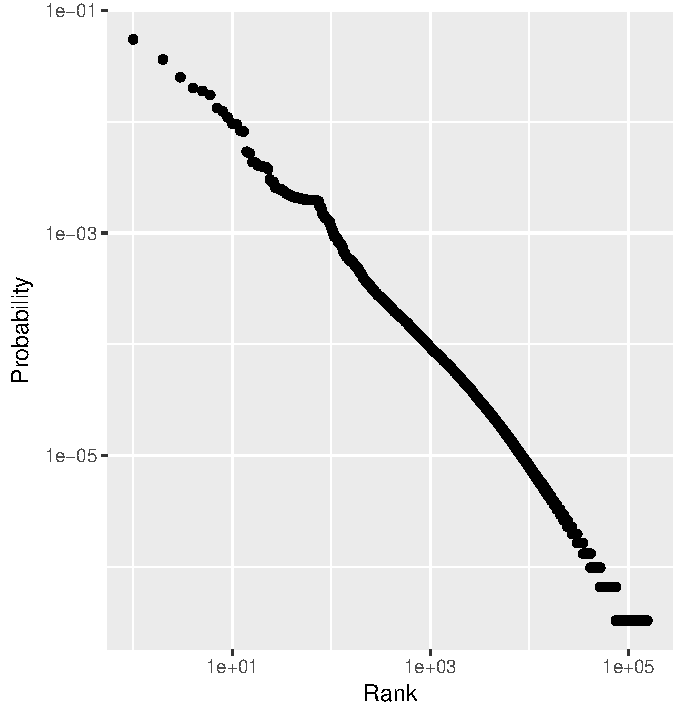
\includegraphics[scale=0.6]{unigram_plot.pdf}
  \caption{Log-log plot of unigram frequency and probability}
  \label{fig:q1p1}
  \end{figure}

   \begin{figure}[h]
  \centering
  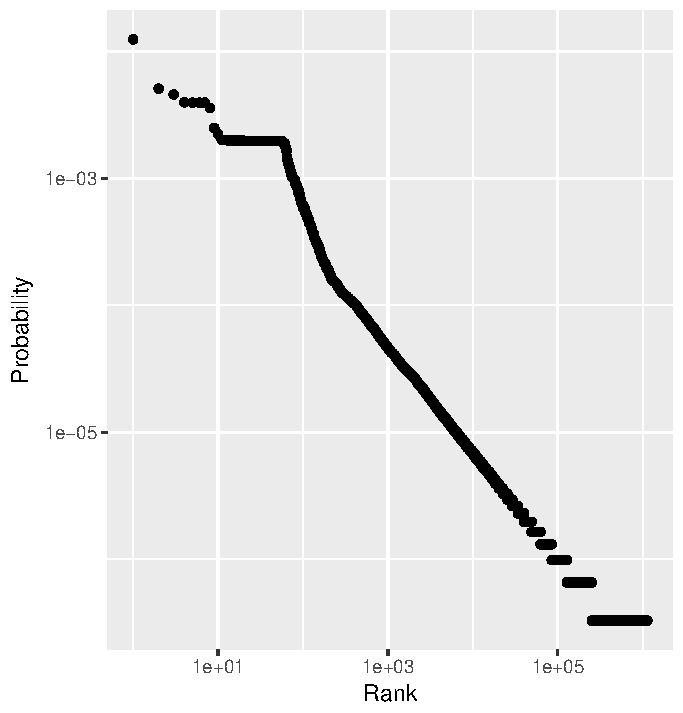
\includegraphics[scale=0.6]{bigram.pdf}
  \caption{Log-log plot of bigram frequency and probability}
  \label{fig:q1p2}
  \end{figure}
  
   \begin{figure}[h]
  \centering
  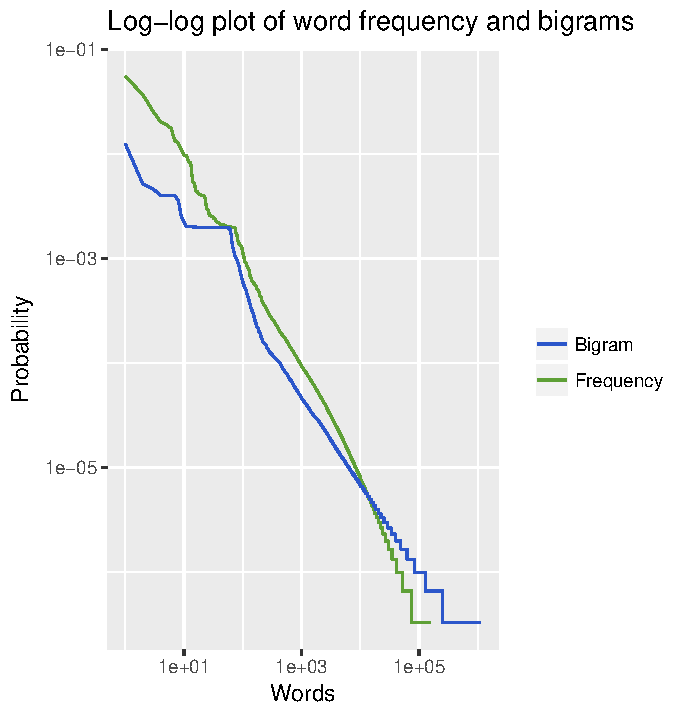
\includegraphics[scale=0.9]{unigram_and_bigram.pdf}
  \caption{Log-log plot of unigram and bigram frequencies and probabilities}
  \label{fig:q1p3}
  \end{figure}


\clearpage

% =================================
% Second question
% =================================

\section*{2}

\subsection*{Question}

\begin{verbatim}
4.2. Plot vocabulary growth for the Wikipedia collection and estimate 
the parameters for Heaps' law. Should the order in which the 
documents are processed make any difference?
\end{verbatim}

\subsection*{Answer}

To answer this question I again created two files, \textbf{vocabGrowth.py} and \textbf{vocabGrowth.R}.
My python script use the Beautifulsoup library to parse out the html documents of the small wikipedia example.
Much like my answer to the first question I traversed the html documents in order and then in reverse, each time tokenizing the text of html, taking an overall corpus count,  tracking unique vocabulary through each of the html documents, and then saving all of these values to csv file denoting document iteration, corpus size, and vocab size when at that document.
The code for this is shown in Listing \ref{lst:q2py}.
The goal of this was simply see how the unique vocabulary list grows while the corpus size continues to grow.

  \lstinputlisting[frame=single,caption={Python script to track vocabulary growth},label=lst:q2py,captionpos=b,numbers=left,showspaces=false,showstringspaces=false,basicstyle=\footnotesize]{\srcPath/vocabGrowth.py}

The relationship between corpus size and vocabulary size was defined in our book as: \[ v = k * n^\beta \]
To estimate the parameters for heaps law and plot the vocabulary growth, I used R's ggplot2 to create charts and the built in function non-linear least squares (nls) as shown in Figure \ref{lst:q2r}.
The parameters of K and B were initialized with a value of one. 
The plot of documents traversed in order is shown in Figure \ref{fig:q2p1} and the plot of the documents traversed in reverse is shown in Figure \ref{fig:q2p2}.
The plots show vocab count along the y-axis and corpus word count along x-axis.
It is apparent that these two graphs are different and that means the order in which the documents are processed does make a difference.

The estimation parameters for Heap's law for in order and reverse, computed by the nls method in R, are shown in Table \ref{table:heap}. 
Some of values do differ slightly, such as the B values for ascending and descending, but there is an apparent difference which further supporting my claim.

\lstinputlisting[frame=single,caption={R script to compute Heap's Law},label=lst:q2r,captionpos=b,numbers=left,showspaces=false,showstringspaces=false,basicstyle=\footnotesize]{\srcPath/vocabGrowth.R}

\begin{table}
\centering
\begin{tabular}{|l|l|l|}
\hline
\multicolumn{1}{|c|}{\textbf{Number}} & \multicolumn{1}{c|}{\textbf{Parameter}} & \multicolumn{1}{c|}{\textbf{Values}} \\ \hline
1 & Document Count & 6043 \\ \hline
2 & K ascending & 7.6679986 \\ \hline
3 & B ascending & 0.6652129 \\ \hline
4 & K descending & 6.276427 \\ \hline
5 & B descending & 0.678342 \\ \hline
\end{tabular}
\caption{Heap's Law parameters for Small Wiki}
\label{table:heap}
\end{table}

   \begin{figure}[h]
  \centering
  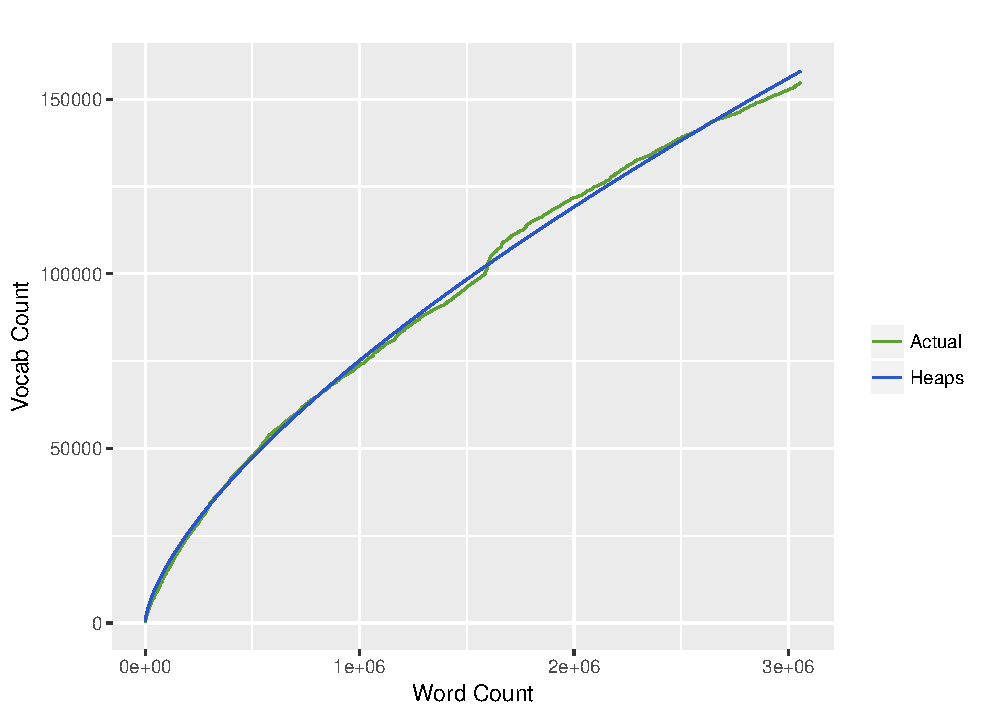
\includegraphics[scale=0.7]{corpusGrowth.pdf}
  \caption{Growth of vocabulary vs overall corpus}
  \label{fig:q2p1}
  \end{figure}
  
   \begin{figure}[h]
  \centering
  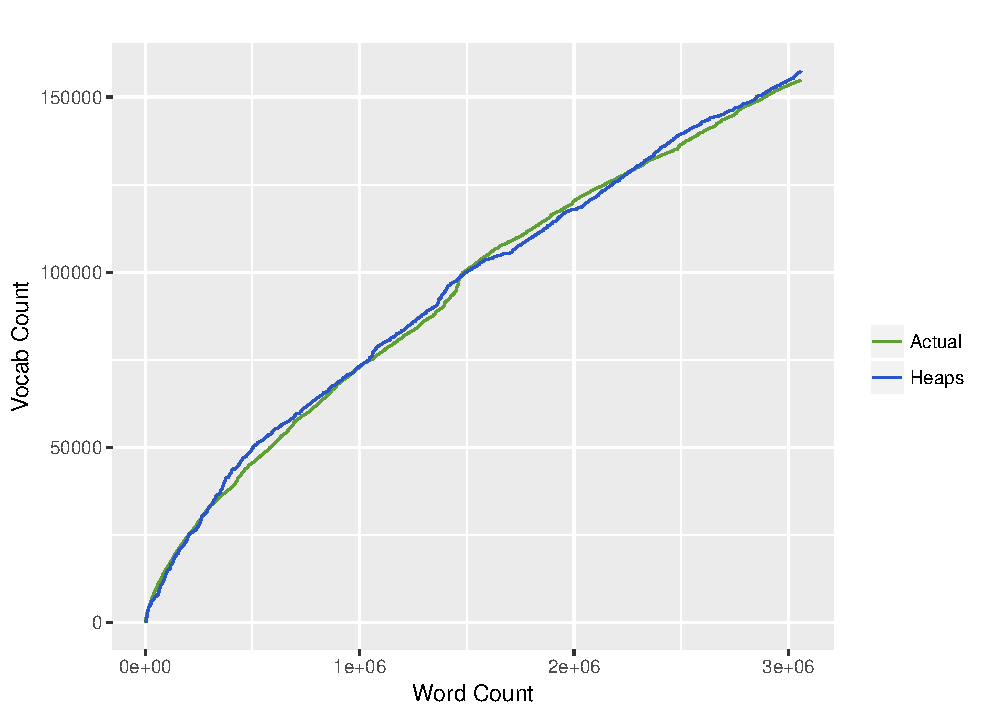
\includegraphics[scale=0.7]{corpusGrowthReverse.pdf}
  \caption{Growth of vocabulary vs overall corpus with documents traversed in reverse}
  \label{fig:q2p2}
  \end{figure}

\clearpage

% =================================
% 3rd question
% =================================

\section*{3}

\subsection*{Question}

\begin{verbatim}
4.3. Try to estimate the number of web pages indexed by two 
different search engines using the technique described in 
this chapter. Compare the size estimates from a range of 
queries and discuss the consistency (or lack of it) of these estimates.
\end{verbatim}

\subsection*{Answer}

The technique described in the textbook \cite{book} is described as follows:

\begin{equation}\label{eq:est}
  f_{ab} = N \cdot f_a/N \cdot f_b/N = (f_a \cdot f_b)/N
\end{equation}

Where:\\
$N$ is the number of documents in the collection.\\
$f_i$ is the number of document that term $i$ occurs.\\
$f_{ab}$ is the combined set result.\\

To estimate $N$ we can use the following equation:
\begin{equation}
	N = \frac{(f_a \cdot f_b)}{f_{ab}}
\end{equation}

The search engines I decided to use in this problem are google and bing. 
My query term for both search engines was ``ocean grove.''
For Google, my variables $f_{a}$, $f_{b}$, and $f_{ab}$ are described as follows:

\begin{equation*}
	f_{ocean} = 1,240,000,000
\end{equation*}

\begin{equation*}
	f_{grove} = 379,000,000
\end{equation*}

\begin{equation*}
	f_{ocean\ grove} = 7,900,000
\end{equation*}

These are shown in Figures \ref{fig:q3g1}, \ref{fig:q3g2}, and \ref{fig:q3g3} respectively. To estimate $N$ we use the following formula:

\begin{equation*}
	N = \frac{(1,240,000,000 \cdot 379,000,000)}{7,900,000}
\end{equation*}

\begin{equation*}
	N = 59.5 \ billion
\end{equation*}

\begin{figure}[h]
\centering
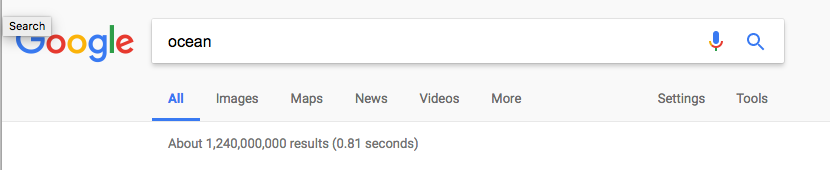
\includegraphics[scale=0.4]{google1.png}
\caption{Google ocean query}
\label{fig:q3g1}
\end{figure}

\begin{figure}[h]
\centering

\includegraphics[scale=0.4]{google2.png}
\caption{Google grove query}
\label{fig:q3g2}
\end{figure}

\begin{figure}[h]
\centering

\includegraphics[scale=0.4]{google3.png}
\caption{Google ocean grove query}
\label{fig:q3g3}
\end{figure}

\clearpage

Comparing this estimated index value to what is shown on the \url{http://www.worldwidewebsize.com/}, as shown in Figure \ref{fig:q3gwww}, its an approximately 59.5/47.2 or 
1.26:1 ratio.

\begin{figure}[h]
\centering
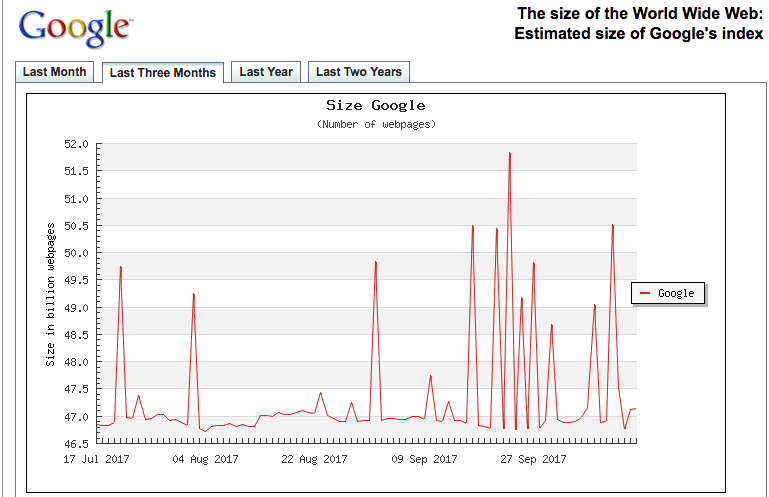
\includegraphics[scale=0.4]{googlewww.png}
\caption{Google's webpage size}
\label{fig:q3gwww}
\end{figure}

For Bing, my variables $f_{a}$, $f_{b}$, and $f_{ab}$ are described as follows:

\begin{equation*}
	f_{ocean} = 183,000,000
\end{equation*}

\begin{equation*}
	f_{grove} = 90,900,000
\end{equation*}

\begin{equation*}
	f_{ocean\ grove} = 296,000
\end{equation*}

These are shown in Figures \ref{fig:q3b1}, \ref{fig:q3b2}, and \ref{fig:q3b3} respectively. To estimate $N$ we use the following formula:

\begin{equation*}
	N = \frac{(183,000,000 \cdot 90,900,000)}{296,000}
\end{equation*}

\begin{equation*}
	N =  56.2 \ billion
\end{equation*}

\begin{figure}[h]
\centering
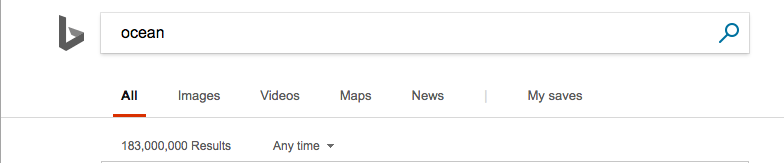
\includegraphics[scale=0.4]{bing1.png}
\caption{Bing ocean query}
\label{fig:q3b1}
\end{figure}

\begin{figure}[h]
\centering
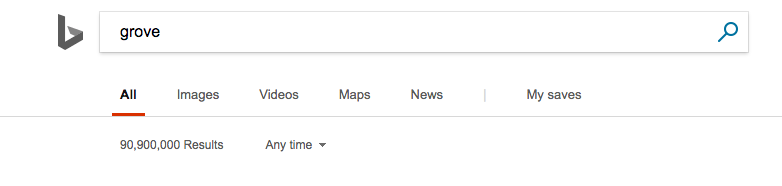
\includegraphics[scale=0.4]{bing2.png}
\caption{Bing grove query}
\label{fig:q3b2}
\end{figure}

\begin{figure}[h]
\centering
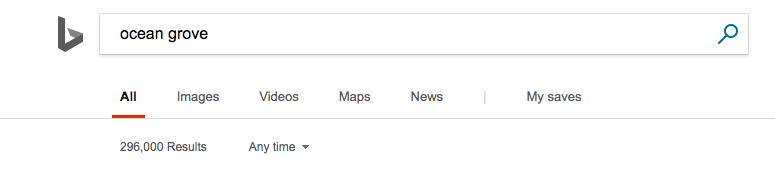
\includegraphics[scale=0.4]{bing3.png}
\caption{Bing ocean grove query}
\label{fig:q3b3}
\end{figure}


Comparing this estimated index value to what is shown on the \url{http://www.worldwidewebsize.com/}, as shown in Figure \ref{fig:q3bwww}, its an approximately 56.2/6 or 
9.37:1 ratio. 
This is a huge difference compared to google.  
It clearly shows that Bing isn't putting as much resources into their search engine as google is.
  
\begin{figure}[h]
\centering
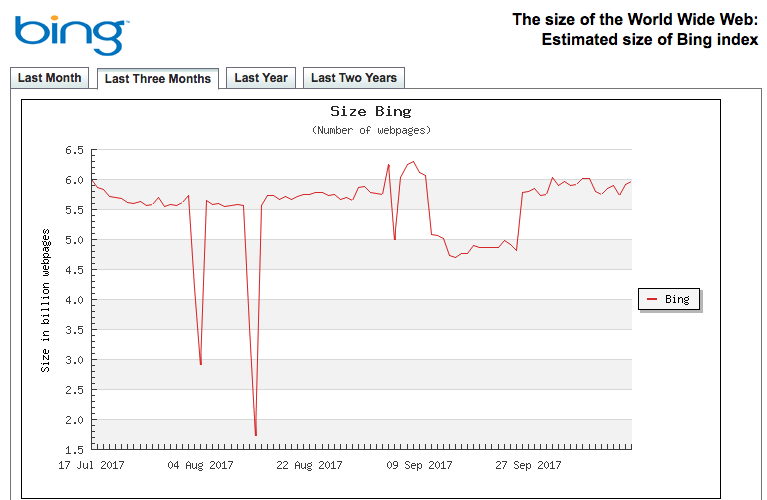
\includegraphics[scale=0.4]{bingwww.png}
\caption{Bing's webpage size}
\label{fig:q3bwww}
\end{figure}

\clearpage

% =================================
% 4th question
% =================================

\section*{4}

\subsection*{Question}

\begin{verbatim}
4.8. Find the 10 Wikipedia documents with the most inlinks. 
Show the collection of anchor text for those pages.
\end{verbatim}

\subsection*{Answer}

To answer this question I wrote a script named \textbf{inlinks.py} as shown in Listing \ref{lst:q4py}.
This script once again takes advantage of Beautifulsoup to parse html, but this time I also used it to extract all the ``a'' element tags with href tags.
For each of the URIs found I would create a dictionary with their destination and their anchor text to the html element.
The results of this is shown below in Table \ref{table:inlink}.
This data is also present on my github page called \textbf{inlinks.csv} in the data directory \cite{github}.
You should probably go to the github, because I can't format my tables properly.

\clearpage

\begin{table}
\begin{tabular}{| l | l | l |}
\hline
\multicolumn{1}{|c|}{\textbf{Link}} & \multicolumn{1}{c|}{\textbf{Inlink Count}} & \multicolumn{1}{c|}{\textbf{Anchor Text}}  \\ \hline
Brazil.html &124 & BRA, Brazil, Article, Brazilian \\ \hline
Foreign\_hostages\_in\_Iraq\_9250.html & 118 & edit, Article \\ \hline
List\_of\_birds\_of\_the\_United \\ \_Arab\_Emirates\_67ef.html & 66 & edit, Article \\ \hline
2007\_New\_York\_Jets\_season\_b663.html & 64 & article, edit, 2007 \\ \hline
German\_railway\_signalling.html & 53 & edit, Article \\ \hline
August\_26.html & 50 & 08-26, 26 August 26, August 26, edit, Article \\ \hline
IPv6\_fdb7.html & 50 & edit, Article \\ \hline
Symmetry.html & 45 & edit, Article \\ \hline
List\_of\_important\_publications \\ \_in\_geology.html & 44 & edit, Article \\ \hline
List\_of\_units\_using\_the\_B-26\_Marauder \\ \_during\_World\_War\_II\_9296.html & 41 & edit, Article \\ \hline
\end{tabular}
\caption{Heap's Law parameters for Small Wiki}
\label{table:inlink}
\end{table}

\lstinputlisting[frame=single,caption={Python script to find top 10 inlinks in small Wiki dataset},label=lst:q4py,captionpos=b,numbers=left,showspaces=false,showstringspaces=false,basicstyle=\footnotesize]{\srcPath/inlinks.py}

\clearpage

% =================================
% 5th question
% =================================

\section*{5}

\subsection*{Question}

\begin{verbatim}
5.8. Write a program that can build a simple inverted 
index of a set of text documents. Each inverted list
will contain the file names of the documents that contain
that word.
Suppose the file A contains the text ``the quick brown fox'', 
and file B contains ``the slow blue fox''. The output of
 your program would be:

\% ./your-program A B
blue B
brown A
fox A B
quick A
slow B
the A B
\end{verbatim}

\subsection*{Answer}

Having done something very similar before for extra in CS532 \cite{cs532}, I decided to lookup some old code I found on a website called Rosetta Code \cite{invertedindexref}.
This code basically is a simple way to create an inverted index.
You first tokenize each html document you call on the command line and build a dictionary of files whose attributes are unique terms and tracking all the unique terms.
You can then iterate through the unique terms and map each file that has the term in the term's dictionary. 
In essence this is an inverted index.
It should be noted that instead of writing to the command prompt the answers, I decided to write it to a CSV file because many documents created many terms.
This CSV can be found in my repository in the data directory \cite{github}.
An example run can be shown in Figure \ref{fig:invertIndex} below, first running the program, then print the top 10 lines of the CSV file.

\begin{figure}[h]
\centering
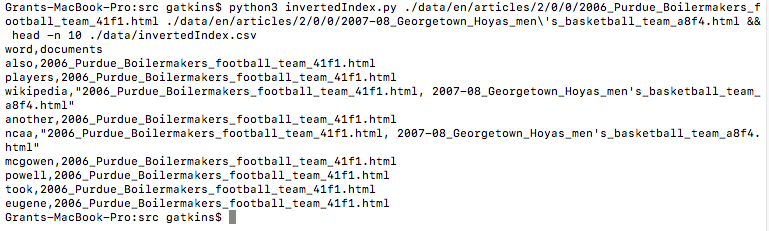
\includegraphics[scale=0.6]{invertedIndexOutput.png}
\caption{Inverted Index sample run with CSV top 10 items}
\label{fig:invertIndex}
\end{figure}

\lstinputlisting[frame=single,caption={Python script to build inverted index from list of files},label=lst:q4py,captionpos=b,numbers=left,showspaces=false,showstringspaces=false,basicstyle=\footnotesize]{\srcPath/invertedIndex.py}

\clearpage


% =================================
% Bibliography
% =================================

\begin{thebibliography}{9}
\bibitem{invertedindexref}
``Inverted Index.'' Roseta Code Inverted index. N.p.,n.d. Web. 22 Feb. 2017. \url{http://rosettacode.org/wiki/Inverted_index#Simple_inverted_index}
\bibitem{cs532}
Atkins, Grant. ``CS532 Assignment 3 Repository'' Github. N.p., 23 March 2017. Web. 23 March 2017.\url{https://github.com/grantat/cs532-s17/tree/master/assignments/A3/src}.
\bibitem{github}
Atkins, Grant. ``CS734 Assignment 2 Repository'' Github. N.p., 21 September 2017. Web. 14 October 2017.\url{https://github.com/grantat/cs834-f17/tree/master/assignments/A2}.
\bibitem{book}
B. Croft, D. Metzler, and T. Strohman. ``Search Engines: Information Retrieval in Practice.'' Pearson, 2009. Web. 14 October 2017. ISBN 9780136072249.
\end{thebibliography}

\end{document}
